During the analysis and planning stages it quickly became apparent that a central authentication and authorization system would be required.  The Gatekeeper service is responsible for providing this, and does so by acting as both an OAuth 2.0 Authorization Server, and an OpenID Connect Identity Provider (IDP).  Such a setup provides a number of benefits, including seamless Single Sign-On (SSO), relative ease of implementation due to the abundance of available libraries, separation of concerns by decoupling authentication \& authorization from each microservice, and the theoretical ability to allow third-party access to AberFitness APIs in the future.

\subsubsection{IdentityServer 4}

Rather than attempting to implement our own OAuth 2.0 server, it seemed beneficial in terms of both security and development time to use an existing solution.  After thorough investigation of the available implementations, IdentityServer 4 was chosen as it not only fully implements the specification of OAuth 2.0 and OpenID Connect, but is also certified by the OpenID Foundation, and is part of the .NET Foundation.  Thorough documentation is available, the project is open-source with a permissive license, and the library is specifically designed for .NET Core 2.

\subsubsection{OAuth Overview}

Two basic OAuth 2.0 flows are used within AberFitness - Authorization Code (including the hybryid flow OpenID Connect extension) for applications with a GUI wishing to identify users, and Client Credentials for API authorization between the various microservices.

When a user first attempts to access a service where authentication is required, they are redirected to Gatekeeper in order to log in.  Once logged in, they are redirected back to the client application which completes a token validation process in order to verify the login.  To facilitie SSO, users which are already logged in to Gatekeeper will be seamlessly redirected back to the client application with no action required from them.

\begin{figure}[H]
    \centering
    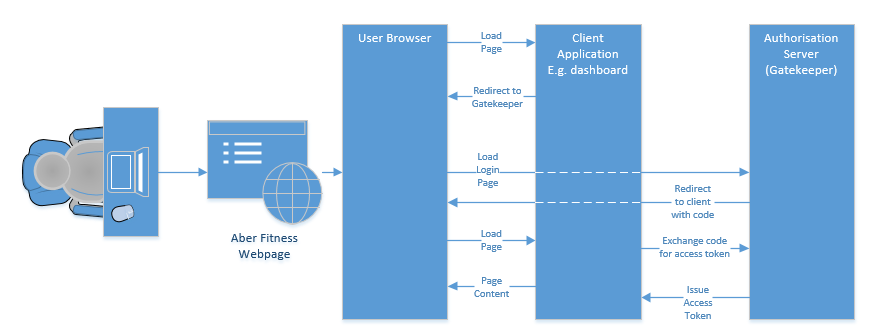
\includegraphics[width=\textwidth]{Images/gatekeeper_authcode_flow.png}
    \caption{Simplified diagram showing overview of the OAuth 2.0 Authorization Code flow.}
\end{figure}

On subsequent requests, a redirect to Gatekeeper is not usually required.  Access tokens are valid for one hour, with the client being able to obtain new tokens via the use of a refresh token.  Redirection to Gatekeeper should only be required if the user has cleared their browser cookies, or those cookies have become invalidated for some reason.

When a microservice wishes to call the API of another microservice, they obtain a client credentials access token from Gatekeeper, and send it in the Authorization header of the request they are making.  Access tokens have a limited number of scopes (services) for which they are valid, and the service receiving the request will reject the token should it not contain the scope required for that service.  Once the content of access token has been checked, the signature of the token is validated using the JSON Web Key Set (JWKS) available from Gatekeeper.  This is essentially a public key which can be used to verify that the access token was indeed issued by Gatekeeper.

\begin{figure}[H]
    \centering
    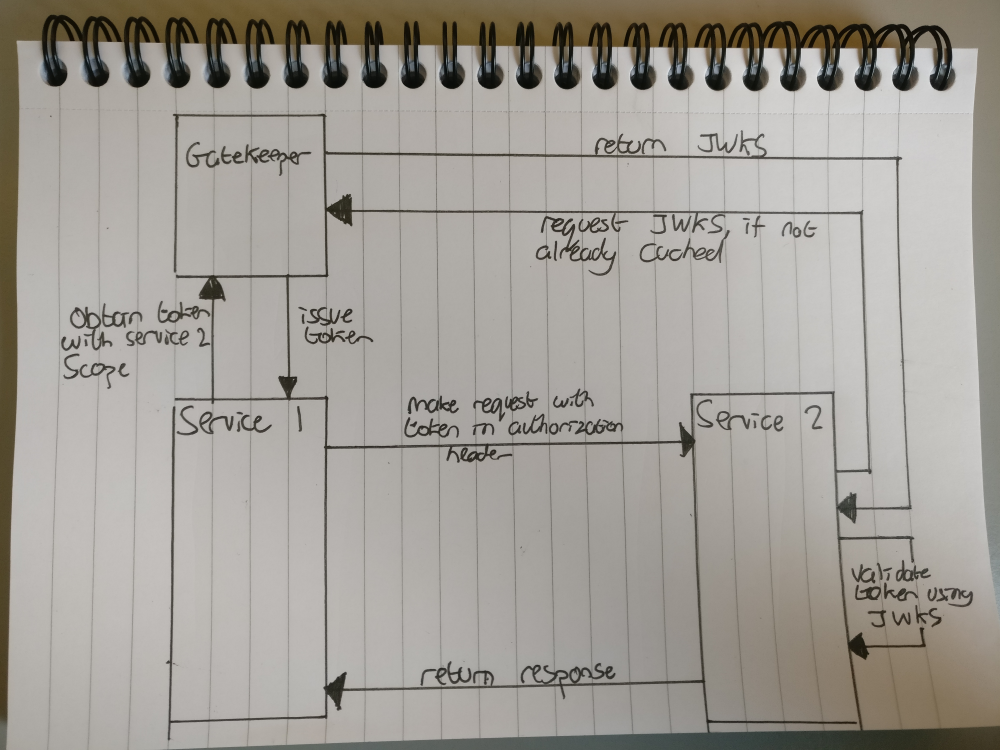
\includegraphics[width=\textwidth]{Images/gatekeeper_clientcredentials_flow.png}
    \caption{Simplified diagram showing overview of the OAuth 2.0 Client Credentials flow.}
\end{figure}

There was some consideration as to whether client credentials was the correct flow to use for authorization when obtaining user resources within AberFitness.  Typically you would require an access token specific to that user, obtained using the authorization code flow, in order to access resources such as activity data belonging to that user.  Eventually it was decided that the authorization code flow would be more relevant to third-party applications wishing to access our APIs.  As all microservices within AberFitness can be considered as belonging to the same overall system, it seemed that the client credentials flow was sufficient to authorize access to data from other services within the AberFitness system.

\subsubsection{Implementation Details}

client libraries

data protection keys

no editing

schema complexity

\subsubsection{Alternatives}

.NET alternatives

Java implementations

SAML

API gateway
